\documentclass[tikz]{standalone}
\tikzset{
  >=latex
}
\begin{document}
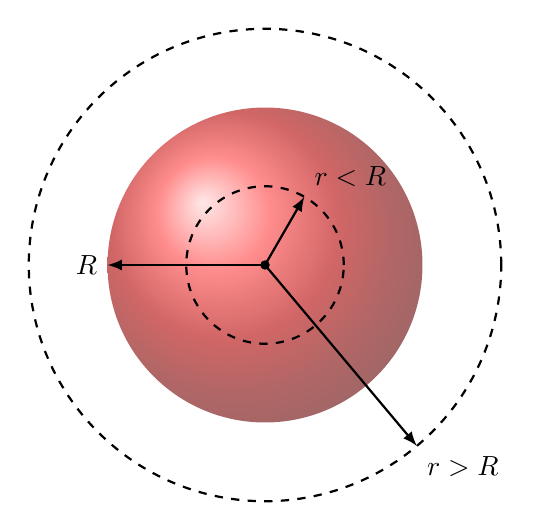
\begin{tikzpicture}[scale=2]
  \shade[ball color=red,opacity=.6](0,0) circle(1);
  \draw[thick,dashed](0,0) circle(.5);
  \draw[thick,dashed](0,0) circle(1.5);
%  \draw[thick,fill=blue!10](0,3.9) arc(90:270:3.9)--(0,-1)
%  arc(270:90:1)--(0,3.9);
%  \draw[thick,fill=blue!18] (0,3.9)arc(90:-90:1.95 and 3.9)--(0,-1)
%  arc(-90:90:.5 and 1)--(0,3.9);
%  \draw[thick,dashed](0,-1) arc(-90:90:1);
  \draw[thick,->,rotate=-50](0,0)--(1.5,0) node[below right]{$r>R$};
  \draw[thick,->](0,0)--(-1,0) node[left]{$R$};
  \draw[thick,->,rotate=60](0,0)--(.5,0) node[above right]{$r<R$};
  \fill(0,0) circle(.03);
%  \draw[thick] (0,3.9)--(0,4);
%  \draw[thick] (0,-3.9)--(0,-4);
%  \node at (3,0) {$-Q$};
%  \node at (-.6,0) {$+Q$};
\end{tikzpicture}
\end{document}
